\documentclass[12pt,a4paper]{article}
\usepackage{fontspec}\usepackage{polyglossia}\setdefaultlanguage{ukrainian}
\setmainfont{NewComputerModern10}\setsansfont{Noto Sans}\setmonofont{Noto Sans Mono}[Scale=.82]
\usepackage{amsmath,amssymb,booktabs,caption,enumitem,float,geometry,graphicx,hyperref,microtype,titlesec,xcolor}
\geometry{left=2cm,right=2cm,top=2cm,bottom=2cm}\setlength{\parindent}{1.25cm}\linespread{1.08}
\titleformat{\section}{\normalfont\fontsize{14}{16}\selectfont\bfseries}{\thesection}{.6em}{}\titlespacing*{\section}{0pt}{1.3em}{.6em}
\titleformat{\subsection}{\normalfont\fontsize{12}{14}\selectfont\bfseries}{\thesubsection}{.6em}{}
\captionsetup{font=small,labelfont=bf,labelsep=endash}
\usepackage[newfloat]{minted}\SetupFloatingEnvironment{listing}{name=Лістинг}
\setminted{fontsize=\footnotesize,linenos,breaklines,autogobble,frame=single,framesep=2mm,bgcolor=gray!5,tabsize=4}
\hypersetup{unicode,colorlinks=true,linkcolor=black,pdftitle={ІО-41, Давидчук А. М., Лабораторна робота №6},pdfauthor={Давидчук А. М.}}
\newcommand{\resultDir}{../results}\newcommand{\studentGroup}{ІО-41}\newcommand{\studentName}{Давидчук А. М.}\newcommand{\reportYear}{2026}
\begin{document}\pagenumbering{gobble}
\begin{titlepage}
\begin{center}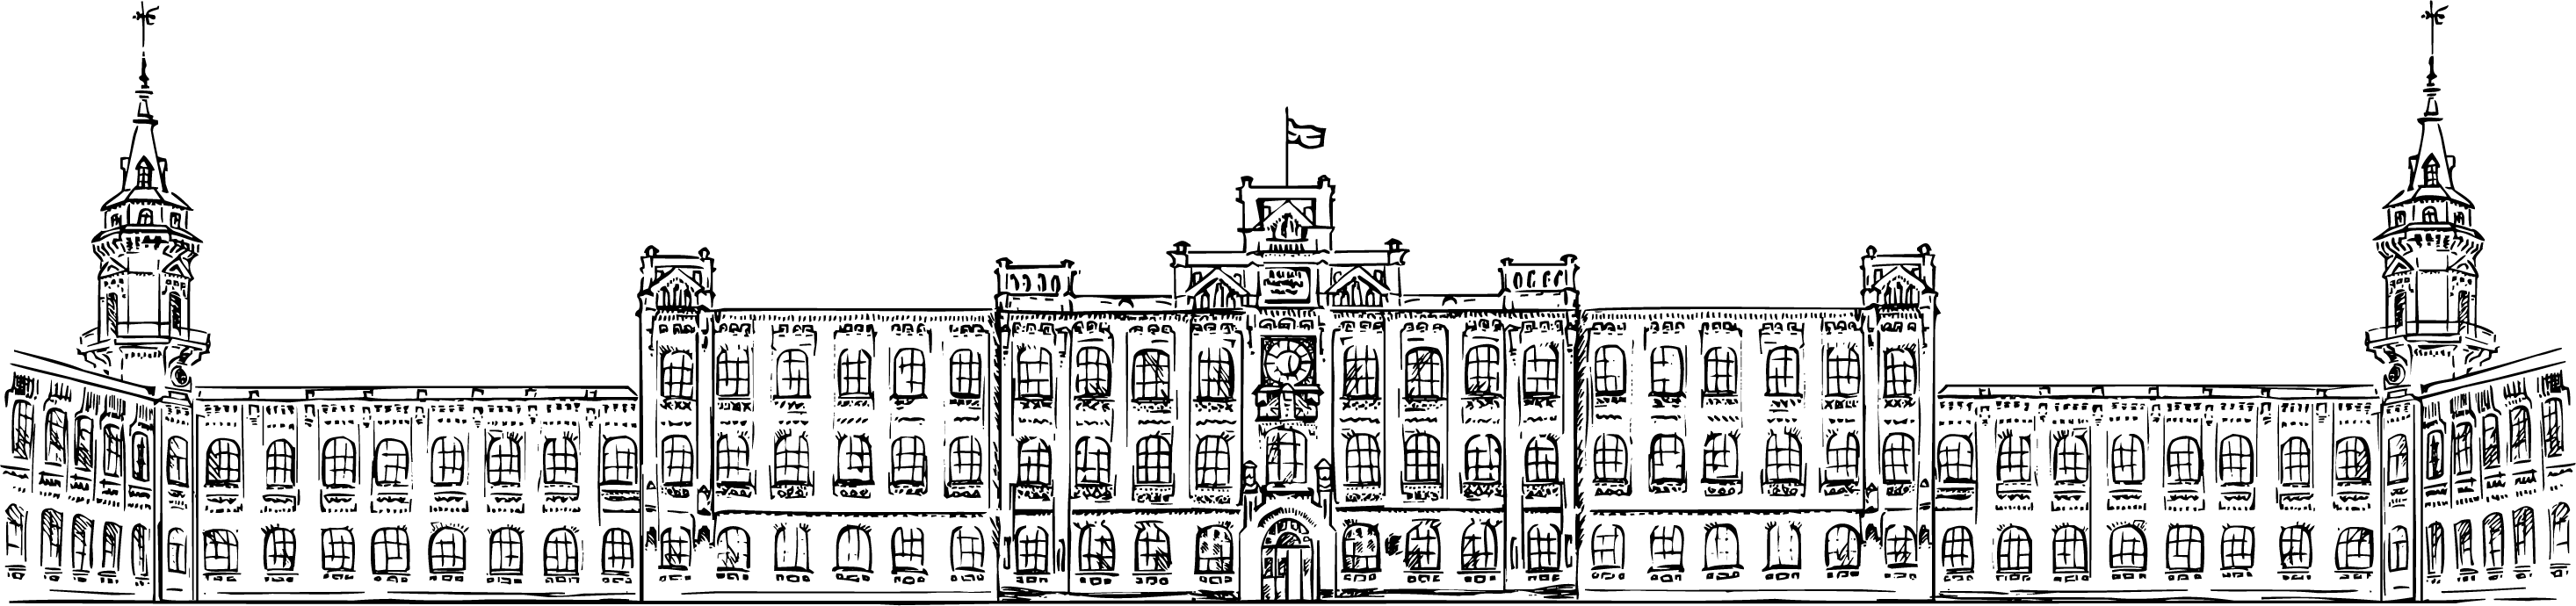
\includegraphics[width=.7\textwidth]{../../../../../../templates/letterhead.png}\end{center}
\begin{center}\large Національний технічний університет України\\ «Київський політехнічний інститут імені Ігоря Сікорського»\\[1em]Факультет інформатики та обчислювальної техніки\\Кафедра обчислювальної техніки\end{center}
\vfill\begin{center}\textbf{\LARGE Методи та технології штучного інтелекту}\\[2em]\textbf{\Large Лабораторна робота №6}\\[.7em]«Нейро-нечітке моделювання»\end{center}
\vfill\begin{flushright}\begin{minipage}{.48\textwidth}Виконав: студент 3 курсу ФІОТ,\\групи \studentGroup\\\textit{\studentName}\\[1em]Перевірив: \textit{Польшакова О. М.}\end{minipage}\end{flushright}
\vfill\begin{center}Київ --- \reportYear\end{center}
\end{titlepage}\pagenumbering{arabic}

\section{Тема та мета роботи}
\noindent\textbf{Тема:} побудова гібридної нейро-нечіткої мережі типу TSK.\\
\noindent\textbf{Мета:} дослідити будову нейро-нечіткої системи, сформувати навчальну вибірку, налаштувати функції приналежності та лінійні наслідки правил, а також перевірити адекватність прогнозу на даних, які модель не бачила під час навчання.

\section{Постановка практичної задачі}
Обрано задачу прогнозування температури процесора за трьома параметрами: завантаженням CPU у відсотках, тактовою частотою в ГГц і швидкістю вентилятора в об/хв. Така задача доцільна для нейро-нечіткого моделювання, оскільки залежність нелінійна, а її логіку можна сформулювати правилами: високе навантаження і висока частота збільшують температуру, а швидке обертання вентилятора її зменшує.

Сформовано 650 прикладів у межах: навантаження $5\ldots100\%$, частота $1{,}2\ldots4{,}4$ ГГц, вентилятор $900\ldots3600$ об/хв. До температури додано невеликий випадковий шум, який імітує похибки датчика та вплив неврахованих факторів. 520 прикладів використано для навчання, 130 --- для незалежного тестування.

\section{Теоретичні відомості}
Нейро-нечітка мережа поєднує інтерпретовані правила нечіткої логіки зі здатністю нейронної мережі підбирати параметри за даними. У моделі Такагі--Сугено--Канга правило має вигляд
\begin{equation}
R_k:\quad \text{якщо }x_1\text{ є }A_{k1},\ldots,x_n\text{ є }A_{kn},\text{ то }f_k=p_{k0}+\sum_{j=1}^{n}p_{kj}x_j.
\end{equation}
Для фазифікації використано гаусові функції
\begin{equation}\mu_{kj}(x_j)=\exp\!\left[-\frac12\left(\frac{x_j-c_{kj}}{\sigma_{kj}}\right)^2\right],\end{equation}
де $c$ --- центр, а $\sigma$ --- ширина. Рівень активації правила дорівнює добутку ступенів належності:
\begin{equation}w_k=\prod_{j=1}^{n}\mu_{kj}(x_j),\qquad \bar w_k=\frac{w_k}{\sum_r w_r}.
\end{equation}
Підсумковий прогноз є зваженою сумою лінійних наслідків:
\begin{equation}\hat y=\sum_k\bar w_k f_k.\end{equation}

Архітектуру можна розглядати як п'ять шарів: фазифікація; обчислення сили правил; обчислення наслідків TSK; сумування; нормалізація й формування виходу. На відміну від звичайної нейромережі, тут можна дослідити активні правила і зрозуміти, чому отримано певний прогноз.

\section{Структура та навчання моделі}
Для кожного з трьох входів використано дві гаусові функції приналежності: умовно «низьке» та «високе» значення. Повний перебір комбінацій утворює $2^3=8$ правил. Перед навчанням входи стандартизуються, тому параметри функцій приналежності мають порівнюваний масштаб.

Навчання є гібридним. За фіксованих центрів і ширин коефіцієнти лінійних наслідків знаходяться регуляризованим методом найменших квадратів. Після цього центри й ширини трохи змінюються; варіант приймається, якщо зменшує MSE на контрольній частині вибірки. Виконано 35 епох зі спадним кроком зміни premise-параметрів. Після вибору функцій приналежності лінійні коефіцієнти повторно обчислюються на всіх 520 навчальних прикладах.

\begin{figure}[H]\centering\includegraphics[width=.96\textwidth]{\resultDir/architecture.png}\caption{П'ять функціональних етапів гібридної мережі TSK}\end{figure}

Повна база нечіткого виводу складається з восьми правил. Позначення Н і В означають відповідно низький та високий терми. Для кожного правила наслідок має лінійну форму $f_k=p_{k0}+p_{k1}x_1+p_{k2}x_2+p_{k3}x_3$.
\begin{table}[H]\centering\small
\begin{tabular}{ccccc}\toprule Правило & Навантаження & Частота & Вентилятор & Наслідок\\\midrule
$R_1$ & Н & Н & Н & $f_1$\\
$R_2$ & Н & Н & В & $f_2$\\
$R_3$ & Н & В & Н & $f_3$\\
$R_4$ & Н & В & В & $f_4$\\
$R_5$ & В & Н & Н & $f_5$\\
$R_6$ & В & Н & В & $f_6$\\
$R_7$ & В & В & Н & $f_7$\\
$R_8$ & В & В & В & $f_8$\\\bottomrule
\end{tabular}\caption{База правил нейро-нечіткої системи}\end{table}

\section{Програмна реалізація}
Обчислення ступенів належності, сили правил і нормалізації наведено в лістингу.
\begin{listing}[H]
\inputminted[firstline=48,lastline=70]{python}{../src/main.py}
\caption{Фазифікація, активація правил і навчання наслідків TSK}
\end{listing}

Пошук premise-параметрів виконується з контролем помилки на відкладеній частині навчальних даних.
\begin{listing}[H]
\inputminted[firstline=76,lastline=100]{python}{../src/main.py}
\caption{Гібридне налаштування нейро-нечіткої мережі}
\end{listing}

\section{Результати}
\begin{table}[H]\centering
\begin{tabular}{lrr}\toprule Метрика & Навчальна вибірка & Тестова вибірка\\\midrule
RMSE, $^\circ$C & 1,0898 & 1,0799\\
MAE, $^\circ$C & 0,8694 & 0,8313\\
$R^2$ & 0,9918 & 0,9914\\\bottomrule
\end{tabular}\caption{Якість нейро-нечіткого прогнозу}\end{table}

Близькі значення навчальних і тестових метрик свідчать, що модель не перенавчилася. Середня абсолютна помилка на нових даних становить близько $0{,}83^\circ$C, а коефіцієнт $R^2=0{,}9914$ означає, що модель пояснює понад 99\% варіації температури.

\begin{figure}[H]\centering\includegraphics[width=.86\textwidth]{\resultDir/training.png}\caption{Зміна контрольної MSE під час налаштування premise-параметрів}\end{figure}
Крива не зростає, бо нові центри та ширини приймаються тільки за умови покращення. Поступове зменшення кроку дозволяє спочатку досліджувати ширшу область параметрів, а наприкінці уточнювати знайдене рішення.

\begin{figure}[H]\centering\includegraphics[width=.78\textwidth]{\resultDir/membership_functions.png}\caption{Навчені гаусові функції приналежності трьох входів}\end{figure}
Перекриття функцій потрібне для плавного переходу між правилами: один приклад може частково активувати кілька правил, а прогноз змінюється без стрибків.

\begin{figure}[H]\centering\includegraphics[width=.68\textwidth]{\resultDir/prediction.png}\caption{Фактична та прогнозована температура на тестовій вибірці}\end{figure}
Точки розташовані біля діагоналі ідеального прогнозу. Помилки не мають вираженого систематичного зміщення в області низьких або високих температур.

\begin{figure}[H]\centering\includegraphics[width=.9\textwidth]{\resultDir/comparison.png}\caption{Порівняння фактичних і прогнозованих значень}\end{figure}

\section{Висновки}
Побудовано TSK/ANFIS-подібну нейро-нечітку модель із трьома входами, вісьмома правилами та лінійними наслідками. Вона прогнозує температуру CPU за навантаженням, частотою і швидкістю вентилятора. На тестовій вибірці отримано RMSE $1{,}08^\circ$C та $R^2=0{,}9914$. Отже, невелика система правил точно відтворила нелінійну залежність і водночас зберегла зрозумілу структуру нечіткого виводу.

\section{Контрольні питання}
\begin{enumerate}[leftmargin=*]
\item \textit{Що таке нейро-нечітка мережа?}\\
Це гібридна модель, у якій нечіткі функції приналежності та правила налаштовуються за навчальними даними методами, подібними до навчання нейромереж.
\item \textit{У чому головна ідея інтеграції нейромереж і нечітких систем?}\\
Нейромережеве навчання автоматично підбирає параметри, а нечітка система зберігає зрозумілі лінгвістичні правила.
\item \textit{Які компоненти має нейро-нечітка система?}\\
Фазифікатор, база правил, механізм агрегації, блок наслідків, нормалізація та алгоритм навчання.
\item \textit{Які архітектури нейро-нечітких мереж відомі?}\\
Поширені ANFIS/TSK, нейро-нечіткі системи Mamdani, NEFCLASS і моделі з нечіткими нейронами.
\item \textit{Що таке ANFIS?}\\
ANFIS --- адаптивна система нейро-нечіткого виводу, яка реалізує правила Sugeno у вигляді багатошарової мережі.
\item \textit{Які шари виділяють в ANFIS?}\\
Фазифікацію, активацію правил, нормалізацію, обчислення наслідків і сумування виходу.
\item \textit{У чому полягає навчання нейро-нечіткої мережі?}\\
У підборі центрів і ширин функцій приналежності та коефіцієнтів наслідків так, щоб зменшити помилку прогнозу.
\item \textit{Які алгоритми навчання застосовують?}\\
Градієнтний спуск, метод найменших квадратів, гібридні алгоритми та еволюційні методи.
\item \textit{Чим нейро-нечітка мережа відрізняється від класичної нечіткої системи?}\\
Класична система переважно задається експертом, а нейро-нечітка автоматично уточнює параметри за даними.
\item \textit{Які властивості роблять її ефективною?}\\
Нелінійна апроксимація, адаптивність, плавність виводу та інтерпретованість правил.
\item \textit{Яка перевага над звичайною нейронною мережею?}\\
Рішення можна пояснити через активні функції приналежності та правила, а не лише через набір ваг.
\item \textit{Яка перевага над звичайною нечіткою системою?}\\
Параметри не потрібно повністю підбирати вручну: вони адаптуються за навчальною вибіркою.
\item \textit{Які обмеження мають нейро-нечіткі мережі?}\\
Кількість правил швидко зростає з кількістю входів, а якість залежить від репрезентативності даних.
\item \textit{Чому інтерпретованість правил важлива?}\\
Вона дозволяє перевірити логіку рішення, знайти суперечливі правила й обґрунтувати прогноз користувачу.
\item \textit{Де застосовують нейро-нечіткі мережі?}\\
У прогнозуванні, керуванні, діагностиці, оцінюванні ризику, класифікації та системах підтримки рішень.
\item \textit{Як їх використовують в оптимізації?}\\
Модель може швидко наближати складну цільову функцію, після чого оптимізатор шукає найкращі входи вже на цій моделі.
\item \textit{Яка перевага для систем прийняття рішень?}\\
Система одночасно працює з числовими даними, невизначеністю та зрозумілими правилами.
\item \textit{Як гібридна модель працює з невизначеністю?}\\
Часткові ступені приналежності дозволяють активувати кілька правил і плавно поєднати їхні висновки.
\item \textit{Чим Mamdani відрізняється від Sugeno?}\\
У Mamdani наслідок є нечіткою множиною і потребує дефазифікації; у Sugeno наслідок задається числом або функцією входів.
\item \textit{Які перспективи розвитку нейро-нечітких систем?}\\
Автоматичне скорочення баз правил, поєднання з глибокими мережами, потокове навчання та пояснюваний штучний інтелект.
\end{enumerate}
\end{document}
